



\section{Infrastructure}\label{sec:infra}
The algorithmic architecture of the Ling 2.0 model theoretically provides a technical roadmap for low-cost scaling, while also ensuring the upper limits of training and inference efficiency. 
However, algorithm design alone is insufficient to achieve our objectives. 
Without any engineering optimizations, this highly sparse MoE architecture offers no performance advantage over dense models.
Therefore, we require matching infrastructure capabilities to support efficient training and scale the model to the trillion-parameter level at minimal cost. 
Despite steady progress in LLMs training technologies, building systems that can support efficient trillion-parameter training still presents numerous significant challenges:

\begin{figure}
    \centering
    \includegraphics[width=0.5\linewidth]{figs/Infra_overview.png}
    \caption{The overview of the optimization tasks we implemented for \texttt{Ling-1T} during the pretrain stage.}
    \label{fig:infra_overview}
\end{figure}






\textbf{FP8 Training.}
To reduce the training cost of the Ling 2.0 model and enhance its efficiency in both training and inference, all models are trained entirely in FP8 precision \citep{deepseekai2024deepseekv3technicalreport}, which presents challenges in both precision and stability.
We provide an advanced FP8 training framework that achieves near-lossless model performance, while simultaneously reducing computation and memory consumption.

\textbf{Heterogeneous TransformerBlock.} The MTP block and the First-K-Dense strategy shift the Pipeline Parallelism (PP) scheduling units from homogeneous to heterogeneous, implying that the forward and backward computational latencies as well as memory consumption may differ across blocks, which can significantly increase pipeline bubbles without careful design.

\textbf{Increased Number of Experts and Higher Sparsity.} These lead to higher communication costs in Expert Parallelism (EP) and increased CPU overhead.

\textbf{Larger Overall Model Size.} Scaling in model size entails greater computational and memory demands, and increased distributed training overhead.

\textbf{Co-Design of Algorithms and Systems.} Advances in model architectures necessitate effective co-design during the model development phase to ensure maximal utilization of hardware resources.

To address the new challenges, we upgrade our infrastructure, which helps the Ling 2.0 models achieve optimal training and inference efficiency. 
Figure~\ref{fig:infra_overview} summarizes the optimizations, and the specific results are obtained from the \texttt{Ling-1T} training.
Baseline performance is measured under the following configuration: a modified version of Megatron 0.11, the FP8 training strategy adapted to Ling 2.0 with MTP support, running on 2016 $\times$ Hopper GPUs.
Other key distributed training settings include: TP1, EP8, PP21, VPP2, sequence length 4K, and fully recomputation.

\subsection{FP8 Training}

Ling 2.0 employs a fine-grained block-wise FP8 quantization strategy: activations and gradients are quantized in blocks of [1,128] elements, while weights are quantized in blocks of [128,128] elements. During forward and backward passes of most linear layers, the original BF16 tensor is quantized into FP8 E4M3 format along with FP32 scaling factors. 
After FP8 GEMM computation, the output of BF16 is obtained.
Our quantization strategy significantly mitigates the impact of outliers on global quantization errors, making it feasible to train LLMs in FP8. To further ensure FP8 training stability, we use QKNorm introduced in Section~\ref{sec:basic_arch} to prevent the layer-by-layer diffusion of outliers that amplifies quantization errors. 
Simultaneously, our \textbf{FP8 Training Safeguard System} tracks risk coefficients for each operation across all layers in real-time, greatly facilitating timely anomaly detection and intervention. 
Validated on the \texttt{Ling-1T} model, the proposed FP8 mixed-precision framework maintained numerical stability throughout 900B-token training, with a relative loss difference within 0.25\% (averaging around 0.1\%) compared to the BF16 baseline. (as shown in Figure~\ref{fig:ling_bf16_vs_fp8_loss_diff}), with no significant variance on benchmark leaderboards.
On the efficiency side, we reduce CPU overhead through optimizations such as \textbf{Padding Routing Map}, and by employing the \textbf{FP8 On-Demand Transpose Weight} technique to trade time for space, we achieve higher acceleration ratios. Ultimately, FP8 training delivers roughly a +15\% MFU gain for \texttt{Ling-1T}.

\begin{figure}
    \centering
    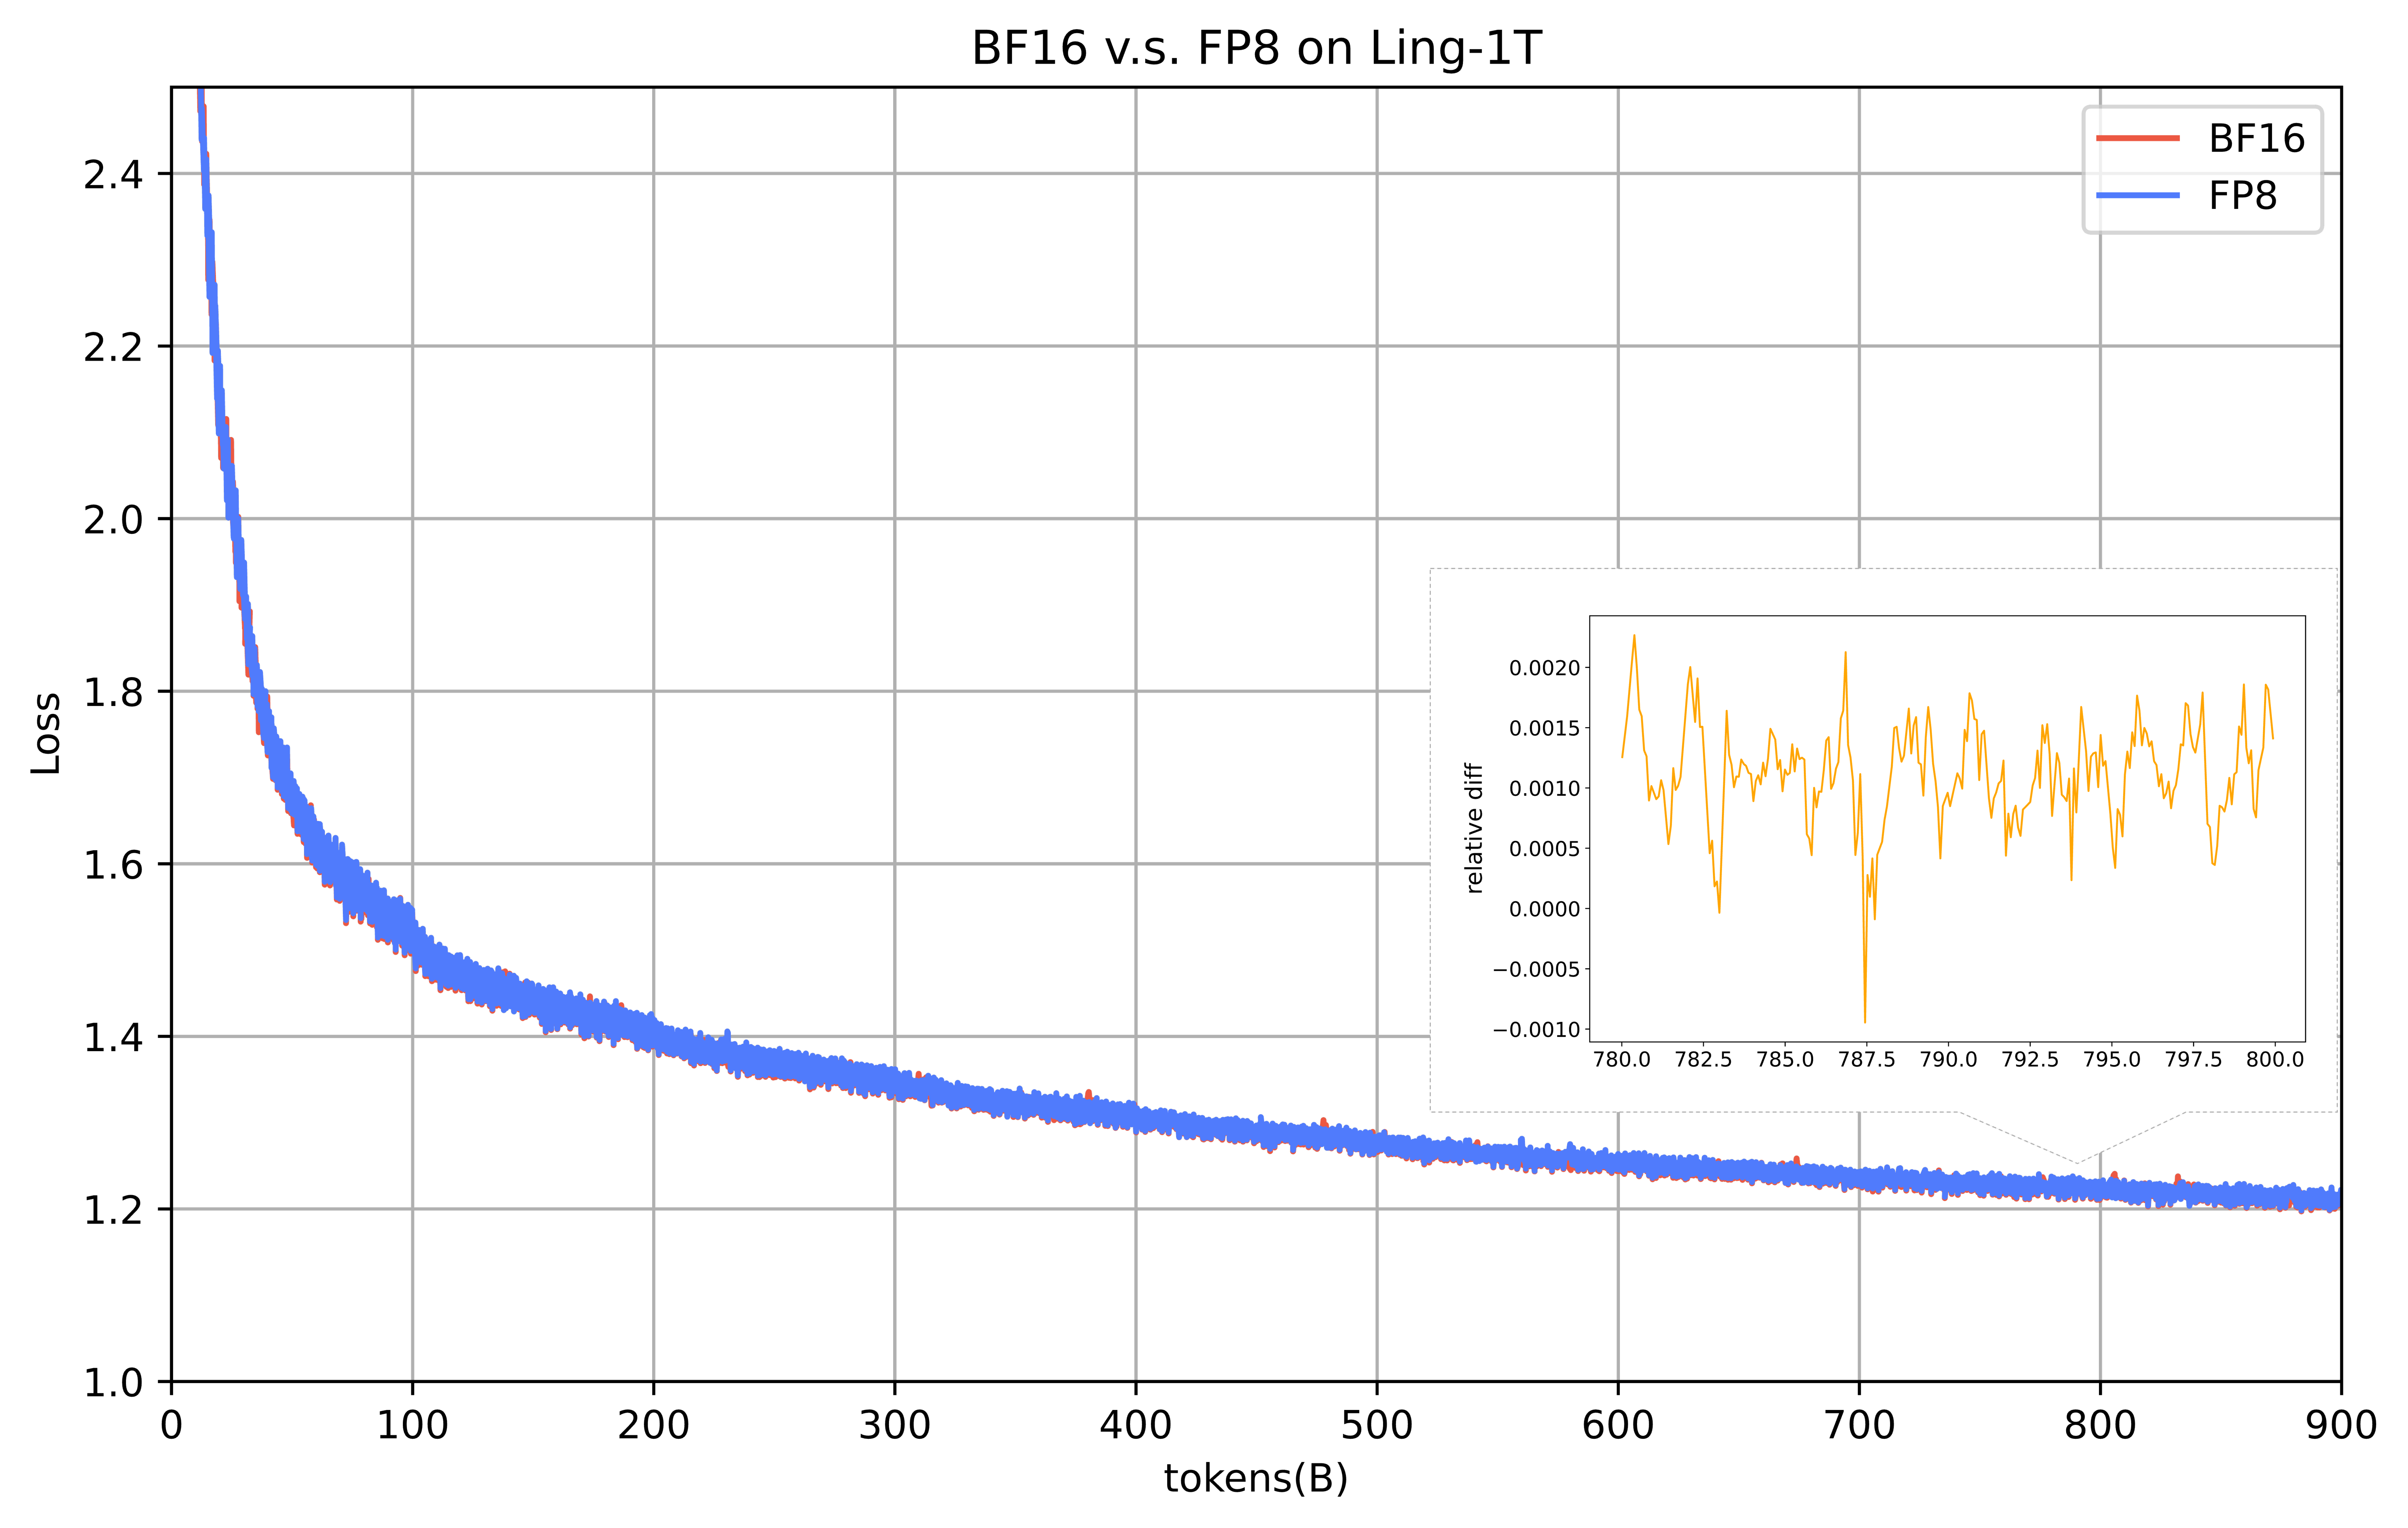
\includegraphics[width=0.58\linewidth]{figs/ling_max_2.0_bf16_vs_fp8_loss_diff.pdf}
    \caption{BF16 v.s. FP8 loss diff on \texttt{Ling-1T}.}
    \label{fig:ling_bf16_vs_fp8_loss_diff}
\end{figure}

\subsubsection{Training Percision Tracking and Assurance}
\paratitle{FP8 Training Safeguard System.}
Benefiting from the FP32 accumulate operation that effectively reduces precision errors in FP8 GEMM computations, 
we attribute the precision deviations in our current FP8 training scheme to two primary sources:
1) FP8 Quantization Underflow, defined as the proportion of matrix elements that become zero after quantization.
2) FP8 Quantization Distortion, a measure of information loss calculated as the cosine similarity between the original and reconstructed (quantized then de-quantized) matrix.
Through error profiling via high-precision recomputation, our FP8 training safeguard system monitors all operations across layers in real time and reports their health status. 
For the first time, we quantify low-precision training safety as measurable indicators, ensuring continuous protection for the training of Ling 2.0 models.

Figure~\ref{fig:ling_fp8_qdq_distortion} shows the trend of FP8 underflow and distortion metrics during the \texttt{Ling-mini-2.0} training process. 
Under the fine-grained FP8 quantization scheme, both activations and gradients maintain healthy precision states, ensuring reliability in forward computations and $\frac{\partial \mathcal{L}}{\partial \mathbf{x}}$ calculations during backpropagation. 
However, monitoring reveals elevated quantization errors in tail layers during gradient transpose computations for $\frac{\partial \mathcal{L}}{\partial \mathbf{W}}$ in backpropagation. 
Through joint analysis with high-precision recomputation metrics and experimental validation, we conclude these errors have negligible impact on model training. 
As $\frac{\partial \mathcal{L}}{\partial \mathbf{W}}$ resides at leaf nodes in the backward propagation path, its quantization errors do not accumulate layer by layer.

\begin{figure}
    \centering
    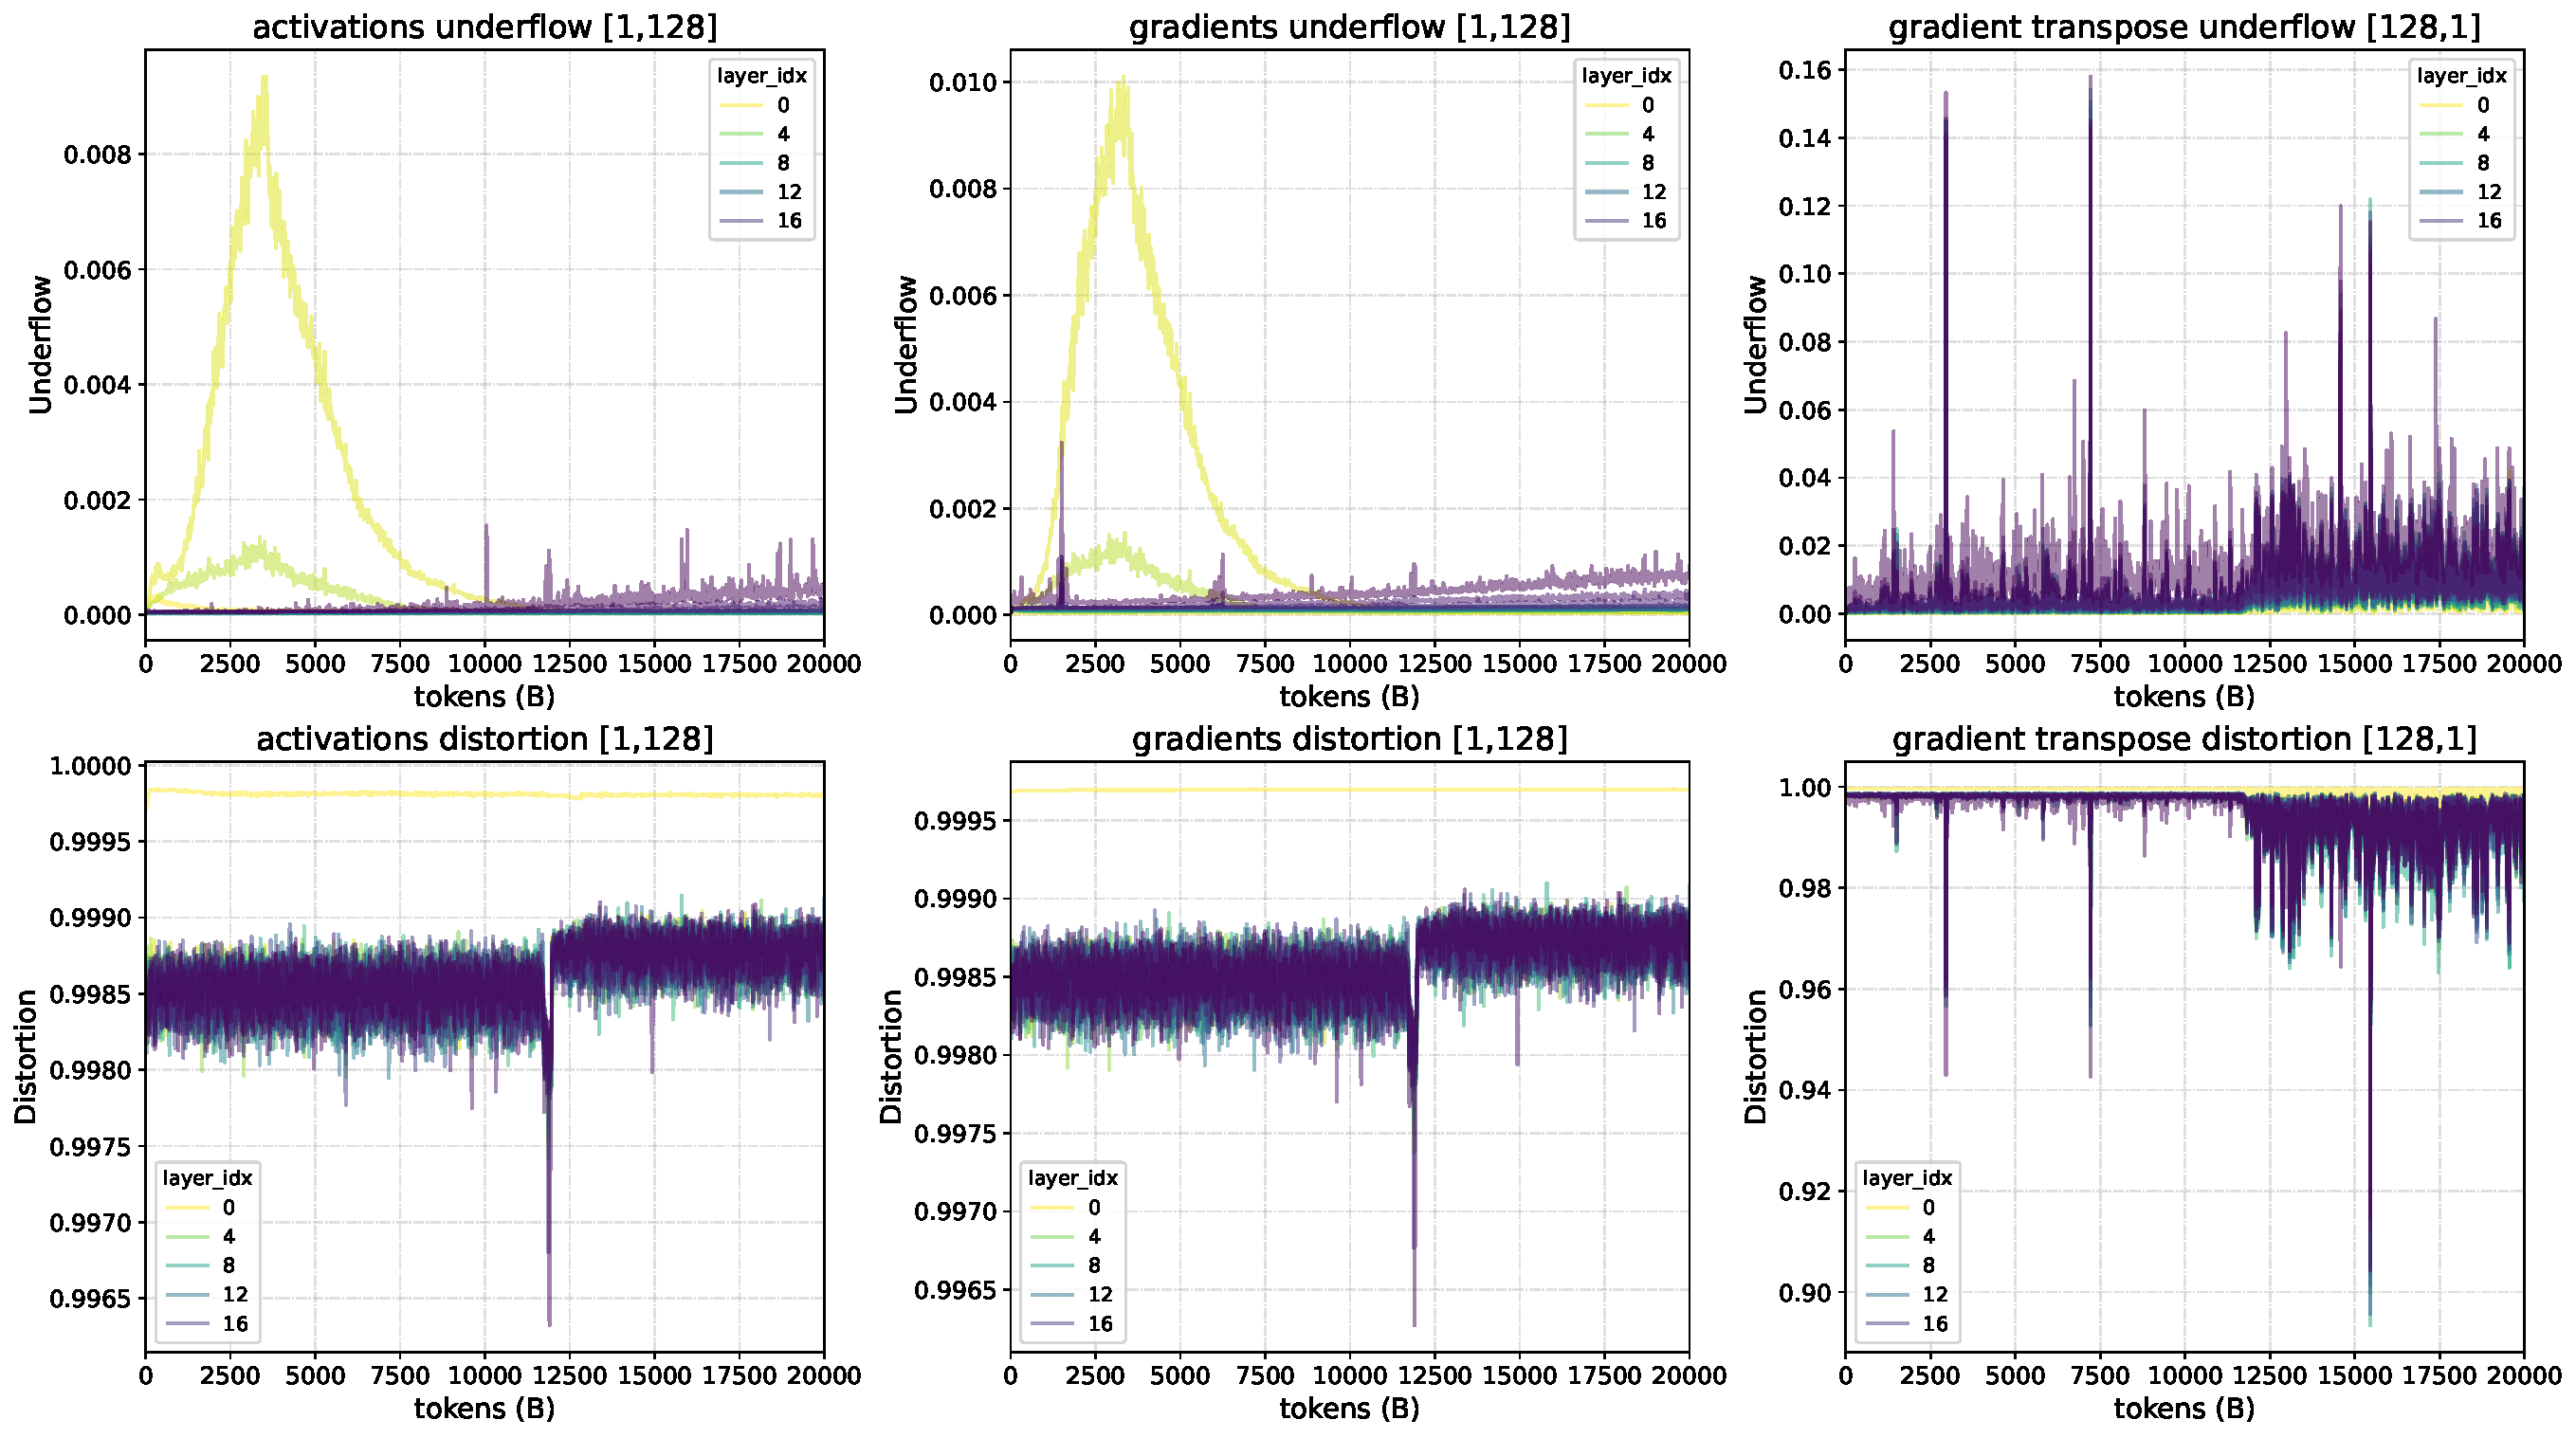
\includegraphics[width=0.8\linewidth]{figs/ling_fp8_qdq_quant_error.pdf}
    \caption{
    FP8 quantization error during pre-training phase of \texttt{Ling-mini-2.0}. For the metrics, a lower underflow is better and higher distortion is better.}
    \label{fig:ling_fp8_qdq_distortion}
\end{figure}

\paratitle{QKNorm to Mitigate Outliers and Reduce FP8 Precision Loss.}
During our early experiments, severe outlier phenomena were observed in both activations and the $\frac{\partial \mathcal{L}}{\partial \mathbf{y}}$ gradient within the \texttt{attention.linear\_qkv} layer. 
These outliers amplify progressively as layer depth increases, directly causing substantial quantization precision errors in FP8 computations for this layer. 
To address this, we introduced QKNorm, which not only suppresses outliers to enhance training stability but also demonstrably reduces precision errors across all FP8 modules in the network.

\subsubsection{Toward Even Greater Training Efficiency}

The computational efficiency of FP8 delivers direct performance gains for end-to-end training. Furthermore, FP8's memory advantages unlock greater flexibility in micro batch size (mbs), parallelization strategies, and recomputation techniques, thereby boosting overall training throughput. To maximize these benefits:
\begin{itemize}[leftmargin=1.5em]
    \item \textbf{CPU Overhead Optimization:} We increase FP8 computation ratio through multiple CPU overhead optimizations (e.g., replacing FP8 padding/unpadding layers with FP8 padding routing map\footnote{https://github.com/NVIDIA/Megatron-LM/commit/92d68dae89af0baab2d4eee092f884902dca4db0}, removing redundant assert checks).
    \item \textbf{Time-Space Tradeoff:} We trade time for VRAM by introducing FP8 on-demand transpose weight \footnote{https://github.com/inclusionAI/linghe} together with the optimizer (\texttt{Ling-mini-2.0} only). Furthermore, our fine-grained FP8 quantization keeps LLM training stable, allowing most tensors to be ``compressed'' and ``decompressed'' at FP8 with negligible error, opening up further ways to reclaim VRAM.
\end{itemize}
By adopting the above techniques, \texttt{Ling-1T} achieves +15\% MFU improvement over BF16 training. On 8/16/32 80GB GPUs, \texttt{Ling-mini-2.0} delivers 30-60\% throughput improvement over LLaMA 3.1 8B and Qwen3 8B when MTP is enabled, and 90-120\% throughput improvement without MTP.

\paratitle{FP8 On-Demand Transpose Weight.}
Due to the low efficiency of FP8 tensor transposition, the Transformer Engine implementation caches an additional pre-transposed weight matrix (weight.T) to accelerate backpropagation. However, this optimization failed to reduce overall memory consumption because the weight are still stored in two copies of FP8 tensors, including the original and transposed forms. To address this, we introduce a high-performance on-demand transpose kernel that eliminates the need for persistent transposed-weight storage, reducing the memory footprint of weight tensors by exactly 50\% without compromising computational correctness.

\paratitle{FP8 Padding Routing Map.}
The FP8 GEMM kernel mandates 16-element alignment for matrix dimensions, a requirement inherently incompatible with dynamic token allocation per expert in Mixture-of-Experts (MoE) architectures. The Megatron implementation addresses this through explicit padding operations, incurring non-negligible CPU overhead. To eliminate this latency, we strategically adjust routing map prior to expert assignment, ensuring resultant tensor dimensions satisfy kernel alignment constraints. As modifications are limited exclusively to zero-probability routing regions, strict mathematical equivalence is preserved, thereby enhancing training throughput without computational side effects.


        

\begin{figure}
    \centering
    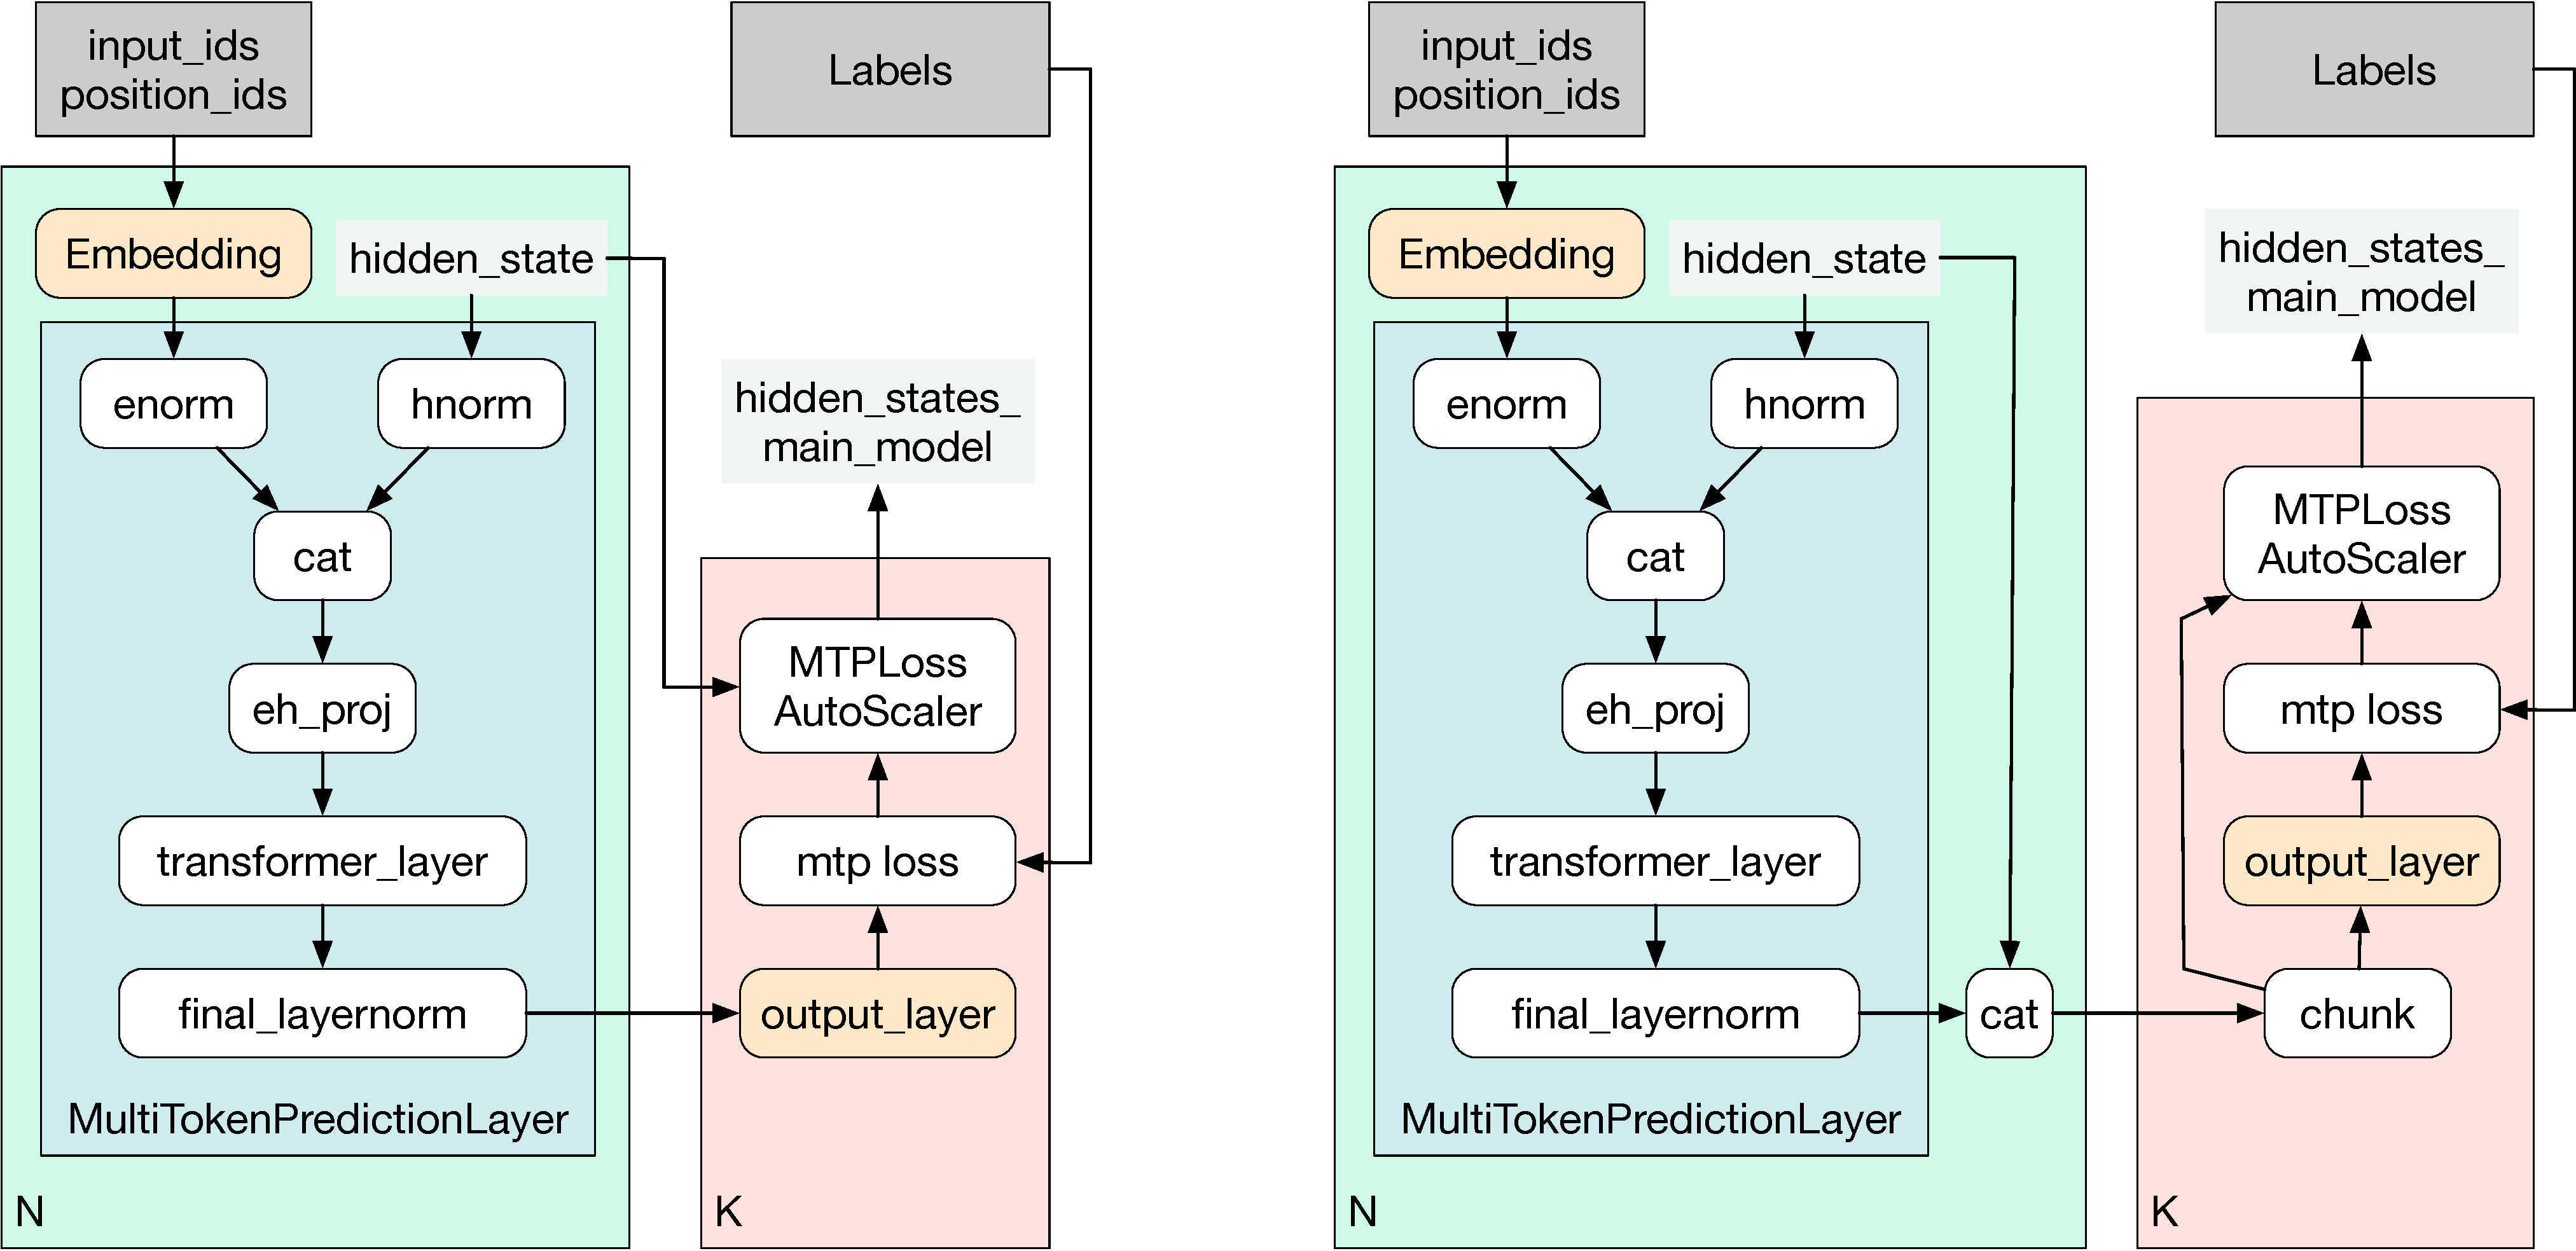
\includegraphics[width=0.7\linewidth]{figs/infra_mtp.pdf}
    \caption{Computation flow before and after the MTP splitting. The left figure shows the original MTP computation flow. The right figure illustrates the computation flow after MTP splitting. In the latter, we divide MTP into individual Transformer layers and a loss computation layer, thereby enabling support for a more fine-grained scheduling scheme.}
    \label{fig:infra_mtp}
\end{figure}

\subsection{Heterogeneous Fine-grained Pipeline Parallelism}
To reduce the bubble ratio in PP, \cite{megatron-lm} proposed the interleaved 1F1B pipeline strategy, and further support features such as non-uniform layer partitioning.
These enhancements aim to alleviate bottlenecks in the first and last stages caused by the presence of Embedding and loss computation layers, which often constrain overall pipeline throughput. Nevertheless, when applying this approach to train the Ling 2.0 series models, we still faced the following challenges:

\begin{itemize}[leftmargin=1.5em]
    \item In addition to the Embedding and loss computation layers, the First-K-Dense strategy and the MTP layers introduced in Ling 2.0 differ significantly from normal MoE layers in both computational and memory consumption, necessitating a more refined PP partitioning strategy.
    \item When employing the interleaved 1F1B pipeline strategy, it is necessary to apply non-uniform partitioning across different PP ranks and VPP stages. This ensures a more balanced workload distribution throughout the pipeline and prevents blocking between stages.
    \item The MTP layer contains $k$ Transformer layers and a loss computation block, both of which incur higher computational and memory cost than a single MoE layer. Furthermore, under the original 1F1B strategy, the MTP layer must be grouped within the same VPP stage alongside another Transformer layer and loss computation layer, causing this stage to become a bottleneck.
\end{itemize}

To address these issues, we modified the PP framework to support the following new features:

\textbf{Configurable Transformer Layer Allocation per VPP Stage:} Enabled flexible configuration of the number of transformer layers per VPP stage, including support for empty stages.

\textbf{Scheduling MTP as a Standalone Layer:} The MTP layer no longer needs to be grouped with other MoE layers or bound to the loss computation layer during scheduling.

\textbf{Partial Recomputation For MTP:} During the backward pass, only the Transformer layer portion within MTP is recomputed, while the logits computation part is not. This approach effectively trades additional memory consumption for improved computation speed.

\textbf{Fine-Grained Partition Strategy For MTP:} Support for partition the MoE layer and the loss computation layer within MTP into two separate layers for scheduling. Figure~\ref{fig:infra_mtp} illustrates the computation flow before and after the MTP splitting operation.

\begin{figure}
    \centering
    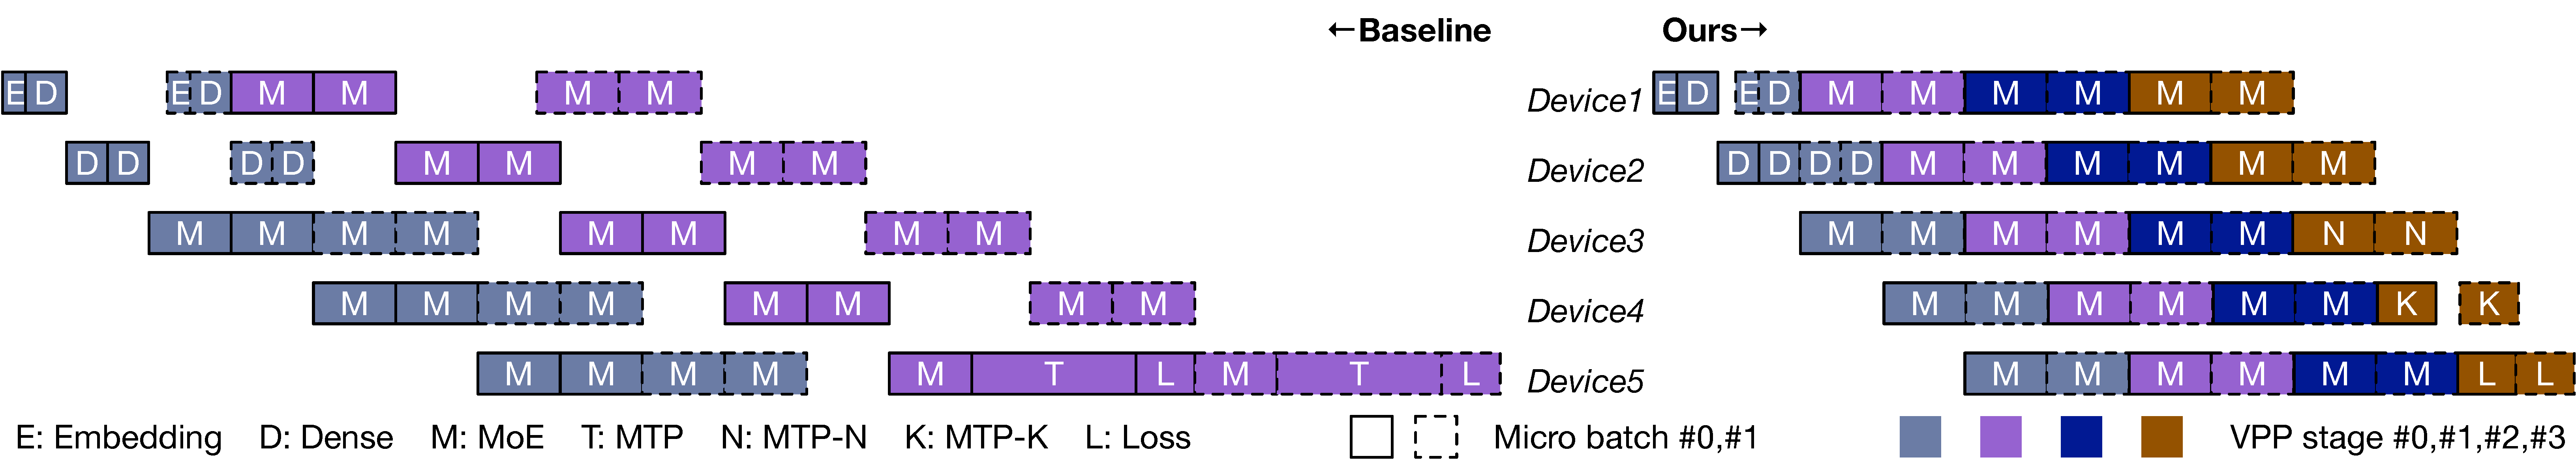
\includegraphics[width=1\linewidth]{figs/heterogeneous_pp.pdf}
    \caption{Example of 1F1B and Heterogeneous Pipeline scheduling for 5 PP ranks. Compared with the baseline, our approach substantially reduces pipeline bubbles, thereby significantly lowering the overall training cost.}
    \label{fig:heterogeneous_pp}
\end{figure}

Figure~\ref{fig:heterogeneous_pp} illustrates the differences in a portion of the forward pass of several micro-batches within the interleaved 1F1B strategy, before and after applying the aforementioned optimizations.
For simplicity, the figure only combines selected segments of the forward step and omits the backward step. The sample model comprises 3 dense layers, 15 MoE layers, and employs 1 MTP layer during training, with a PP size of 5.

In Ling 2.0 training, we observed that the computation cost of a MTP layer is approximately 1.7$\times$ that of a standard MoE layer. Based on this observation, we progressively refined the PP partition strategy, ultimately achieving a 40\% relative end-to-end improvement. 
Furthermore, for MoE models with balanced routing, we can increase virtual pipeline stages from VPP2 to VPP4 to reduce pipeline bubbles, yielding an additional 5\% gain.
However, in other cases where a VPP stage contains only a single MoE layer, the inter-stage blocking becomes more sensitive to imbalanced MoE routing. In such cases, our strategy may not provide end-to-end performance gains.

\subsection{Distributed Training Framework}
In addition to FP8 training and heterogeneous scheduling, we also implement meticulous engineering optimizations on distributed training framework to enhance both performance and stability in Ling 2.0 training.

\subsubsection{Intra-Node DeepEP}
DeepEP \citep{deepseekai2024deepseekv3technicalreport} was designed to optimize EP communication performance across nodes, which reduce significant communication overhead.
During the training of the Ling 2.0 models, we do not involve cross-node EP communication, however, deploying DeepEP for intra-node operations still yields substantial performance gains.
Taking \texttt{Ling-1T} training as an example, the reduction in communication redundancy resulted in a 2\% end-to-end speedup, while operator fusion contributed to an additional 13\% end-to-end performance improvement.


\subsubsection{Fused Kernels}

During the training of Ling 2.0 models, a wide range of fused operators was introduced, including RoPE Fusion, Router Fusion, and Upgrading GroupGemm \citep{megatron-lm}, and others.
Our observations indicate that, in addition to enhancing speed by reducing memory-bound bottlenecks, these fused operators also effectively address substantial CPU overhead encountered during training, which contributes to a notable improvement in end-to-end training performance.

\begin{figure}
    \centering
    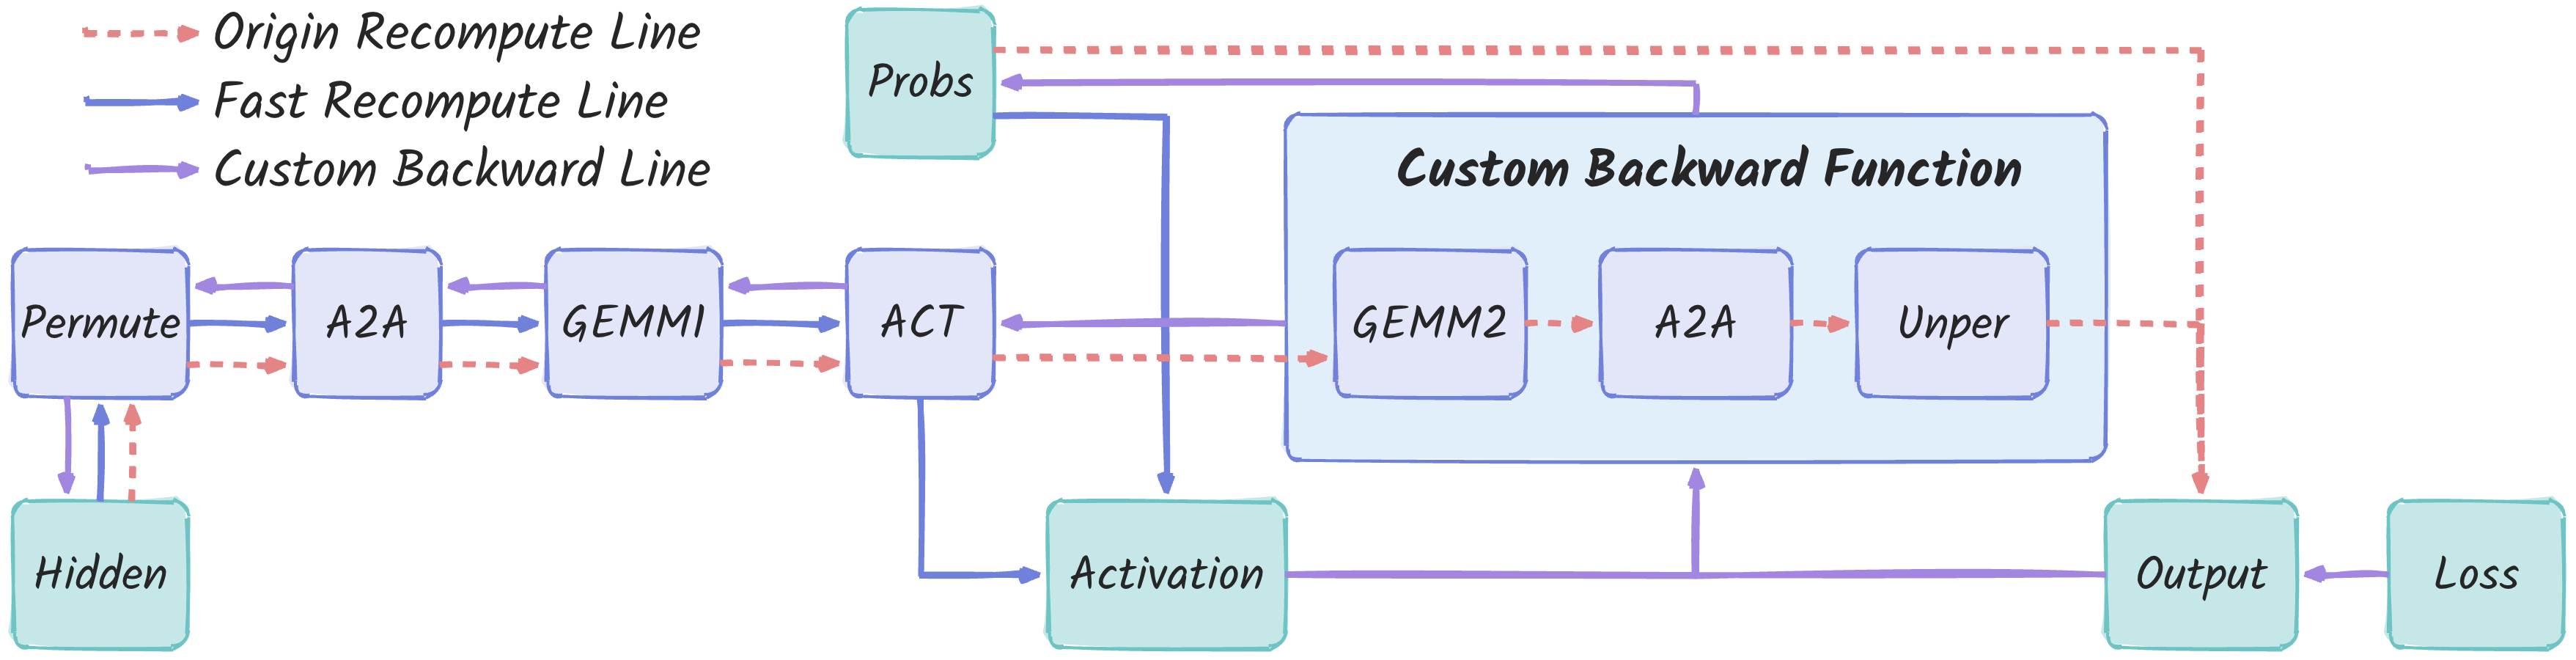
\includegraphics[width=0.8\linewidth]{figs/infra_recompute.png}
    \caption{Illustration of the fast expert recomputation flow.}
    \label{fig:infra_recompute}
\end{figure}

\subsubsection{Fast Expert Full-Recomputation}
To support larger models, we use full recomputation to save GPU memory, enabling larger training within fixed resources at a 25\% compute cost.
Thanks to several recent advances from the community \citep{megatron-lm, mindspeed}, we have identified the potential to reduce recomputation latency by half without incurring any additional cost:

Recent works show that the weighted-sum computation of expert probabilities in the MoE layer can be moved forward to occur within the activation. This eliminates the dependency of the \verb|linear_fc2| and \verb|unpermute| operations on the earlier results in the computation graph.
As illustrated in Figure~\ref{fig:infra_recompute}, unlike standard full-recomputation, we discard the recompute flow before the \verb|linear_fc2|. We then run the backward pass with a custom function for \verb|linear_fc2| and \verb|unpermute|, and propagate its gradients back to activation function to complete the standard backward process.

In Ling‑2.0 training, smaller models saw end‑to‑end performance gains of up to 10\%, while larger models achieved approximately 7\%. The drop is likely due to persistent pipeline bottlenecks in complex partitioning, with some recomputation gains overlapped by pipeline bubbles.

\subsubsection{Long-Context Training}

For LLMs training, long-context training is crucial. In addition to fundamental long-context training techniques, the training process of the Ling 2.0 models has been thoroughly optimized for efficiency in handling long contexts:

\textbf{Long-Context Training with MTP:} We resolved correctness issues related to loss and gradient misalignment when applying Tensor Parallelism (TP) and Context Parallelism (CP) to MTP. This fix enables long-sequence training for Ling 2.0 models with MTP.

\textbf{Support for Cross-Sample Attention Mask:} During long-sequence training, we identified NaN issues in the cross-sample attention mask mechanism, primarily caused by the all-padding issue introduced in the CP implementation. We mitigated these issues in FusedAttention by setting \verb|cu_seqlens_padded| to \verb|cu_seqlens|.

\textbf{Performance Degradation in RoPE Fusion:} In long-context training, varying sub-sequence counts per sample lead to unstable RoPE performance. We mitigate this by limiting sub-sequences and allocating resources based on the actual maximum sequence length per micro-batch, avoiding RoPE performance degradation and fluctuations.

\subsubsection{Framework Optimization}

Beyond MFU optimization, daily token throughput under fixed resources also depends on the Effective Training Time Ratio (ETTR). We address this with the following framework improvements:

\textbf{Optimizing the Storage Latency of Distributed Checkpoints:} 
In Distributed Checkpoint (DCP) saving, GPU Rank0 generates and verifies metadata, which is a time-consuming bottleneck. Since metadata depends solely on the model architecture, we introduced a metadata cache to avoid redundant computation.
For \texttt{Ling-1T}, checkpoint save time dropped from 269s to 30s, and its share of total training time from 2.43\% to 0.82\%.


\textbf{Startup Time Optimization:} To reduce the latency in the job startup phase, we construct a small-scale batch prior to the first forward pass of training.
This batch is passed once through both the forward and backward of the model, allowing all GPU ranks to perform a warm-up computation without storing weights or updating gradients, which reduces the time required for the first training step by approximately 30\%.

\textbf{Optimal Failover Strategy:} To address unrecoverable training failures, checkpoints are periodically saved so that the latest checkpoint can be loaded after a task restart.
A shorter checkpoint interval reduces failover loss, but the saving process incurs non-negligible overhead, making interval configuration critical.
In \texttt{Ling-1T} training, we configure the checkpoint saving interval to be 48 minutes, which is calculated with a simple strategy, and we will discuss it in Appendix~\ref{app:save_interval}.

\textbf{Loss Spike Handling:} Loss spikes can have significant negative impacts on both training stability and model performance. To mitigate these issues, we continued to employ the same methodology utilized in our previous work \citep{team2025every}, monitoring the training state from both the gradient and loss perspectives, and preventing the occurrence of loss spikes.









\subsection{Software Engineering for Foundation LLMs}

During the training of the Ling 2.0 model and the development of the distributed framework, framework development frequently became a bottleneck for model training, and in severe cases could even compromise the training outcomes. Compared with traditional software engineering, we identified the following underlying causes:

\begin{itemize}[leftmargin=1.5em]
    \item \textbf{Unpredictability of Outcomes:} In LLMs development, whether in algorithm or engineering, it is far less predictable than in traditional software. Extensive experiments are needed to improve reliability, but actual testing is often infeasible due to resource limits. Many defects only emerge late in release. Thus, enhancing outcome predictability and early risk detection is essential.
    
    \item \textbf{Trade-offs Between Algorithms and Engineering:} The results from DeepSeek-V3 indicate that only a tight integration of algorithms with software and hardware systems can improve the overall ROI of projects. This requires comprehensive trade-offs in the early stages of model design for certain features, which also increases the complexity of the development process.

    \item \textbf{Diversified Software Deployment Environments:} In both training and inference scenarios, maximizing resource use often involves deployment across heterogeneous hardware. These platforms differ in precision and performance, making alignment of model behavior and efficiency an important research challenge.
\end{itemize}


It is evident that the development process of foundation LLMs involves substantial costs and involves considerable complexity. Therefore, we propose adapting fundamental principles of software engineering to the context of foundation LLMs development, forming a domain we refer to as Foundation LLMs Software Engineering.
We consider Foundation LLMs Software Engineering to be a research domain worthy of in-depth exploration, and further introduce the 4C (Correct, Consistent, Complete, and Co-Design) principle. Its objective is to enhance the efficiency and delivery quality of foundational model development while reducing associated costs.

Based on the 4C principle, we conducted preliminary explorations into several key aspects of foundation LLMs software engineering during the training of Ling 2.0.

\subsubsection{Training Efficiency Optimization and Numerical Integrity Assurance}

The LLMs training cycle typically lasts for several months. Throughout this period, continuous development and iteration of the training framework is needed to improve training efficiency. In addition, we occasionally extend the framework with new functionalities to accommodate algorithmic characteristics or to improve training stability. Throughout the development process, it is essential to ensure the consistency and correctness of model training following these updates.
However, it is nearly impossible to accurately predict the ultimate impact of a planned optimization once deployed to a task running on a large number of GPUs in parallel.

To address this, we have established a workflow for the iterative upgrade of large language model training frameworks, structured as a cycle: Progressive Estimation → Release Approval → Task Monitoring and Sampling Analysis → Experience Accumulation.
During the entire training cycle of a model, experiments are conducted under varying resource configurations, utilizing up to approximately 3\% of the actual training resources. In each iteration, we validate the performance estimation results and only iterations that meet the established standards are approved for release.
For correctness verification, we developed a set of precision alignment and verification tools, which are applied during the development and testing phases. Finally, through continuous observation and analysis of new features, we summarize the corresponding insights and apply them to improve subsequent iterations.


\subsubsection{Co-design of Algorithms and Systems}

\begin{figure}
    \centering
    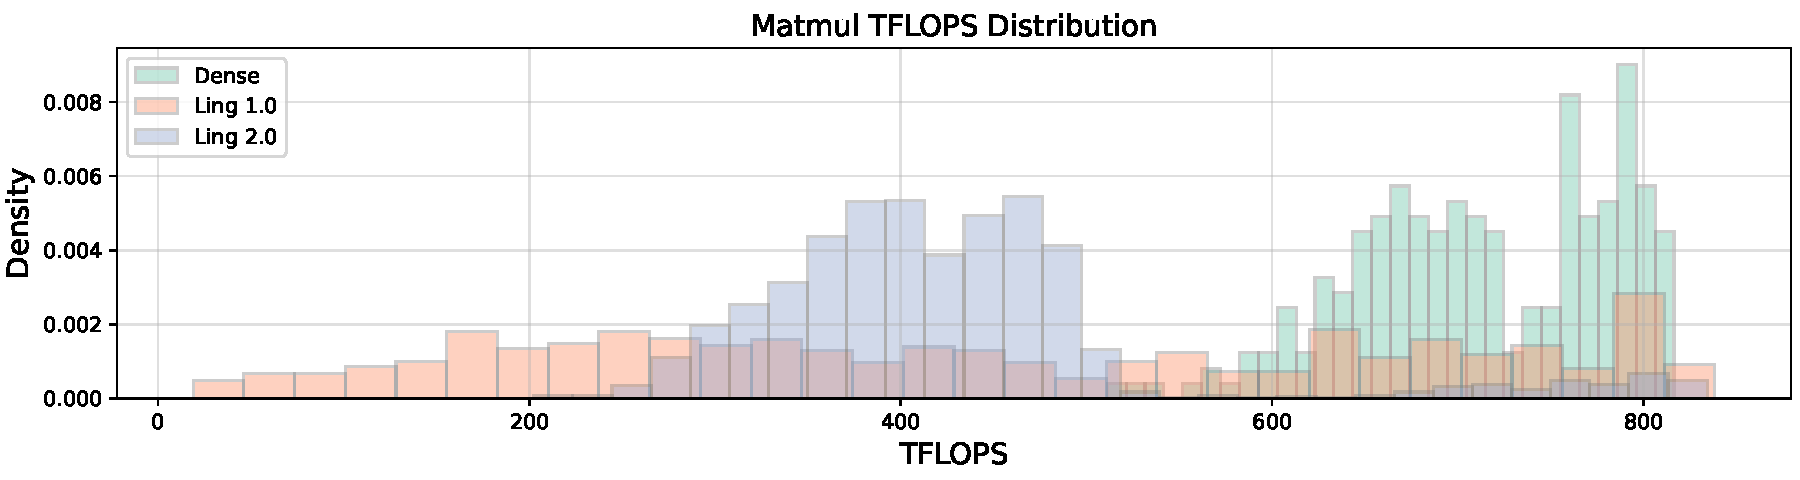
\includegraphics[width=1\linewidth]{figs/infra_flops.pdf}
    \caption{The operator efficiency comparison between the dense architecture, Ling 1.0 and Ling 2.0.}
    \label{fig:infra_op_eff}
\end{figure}

In the development of the Ling 2.0 models, we implemented the following measures to achieve a better trade-off between algorithm performance and system efficiency:


\textbf{Infrastructure-Aware Architecture Design:} 
Taking the Norm Head strategy~\citep{team2025every} as an example, we found that its usage leads to a performance improvement of less than 1\%, while significantly increasing computation and memory consumption within a single PP stage.
This substantial overhead made it challenging to tune the distributed training strategy to an optimal state. Therefore, we did not employ this technique in the training of Ling 2.0 models.
In addition, DeepEP sends a token to up to 4 RDMA and 8 NVLink nodes. To better exploit this feature and prepare for larger-scale EP training in the future, we employ the Group Router algorithm in the MoE layer to divide all experts into 8 groups, and each token is routed within the top 4 scoring groups to maximize intra/inter-node communication efficiency.

\textbf{Operator Efficiency Analysis:} During the design of Ling 2.0, we performed an operator efficiency comparison between the new architecture and Ling 1.0, as shown in Figure~\ref{fig:infra_op_eff}.
Efficiency in Ling‑2.0 is more centered in the mid‑range, consistent with its ``wider and shallower'' design. No operators show exceptionally low efficiency, which we attribute to the First‑K‑Dense strategy mitigating imbalance in shallow MoE layer and improving overall computational efficiency.

\textbf{Parameter Design Integrated with Distributed Architecture:} In the parameter design of Ling 2.0, we carried out detailed parameter configuration tailored to various heterogeneous modules. For example, in the design of \texttt{Ling-1T}, the computation consumption ratio between dense layers and MoE layers was set at 1:2.
This design facilitates achieving uniform computation time across all PP stages, allowing us to minimize pipeline bubbles to the greatest extent possible.

\subsubsection{Cross-Platform Alignment}


During the training process, in addition to using the standard Hopper architecture, we occasionally have the need to train on other heterogeneous GPU.
Throughout this process, we adhere to the 4C principle to align algorithmic logic and results as closely as possible across different platforms.

\begin{figure}
    \centering
    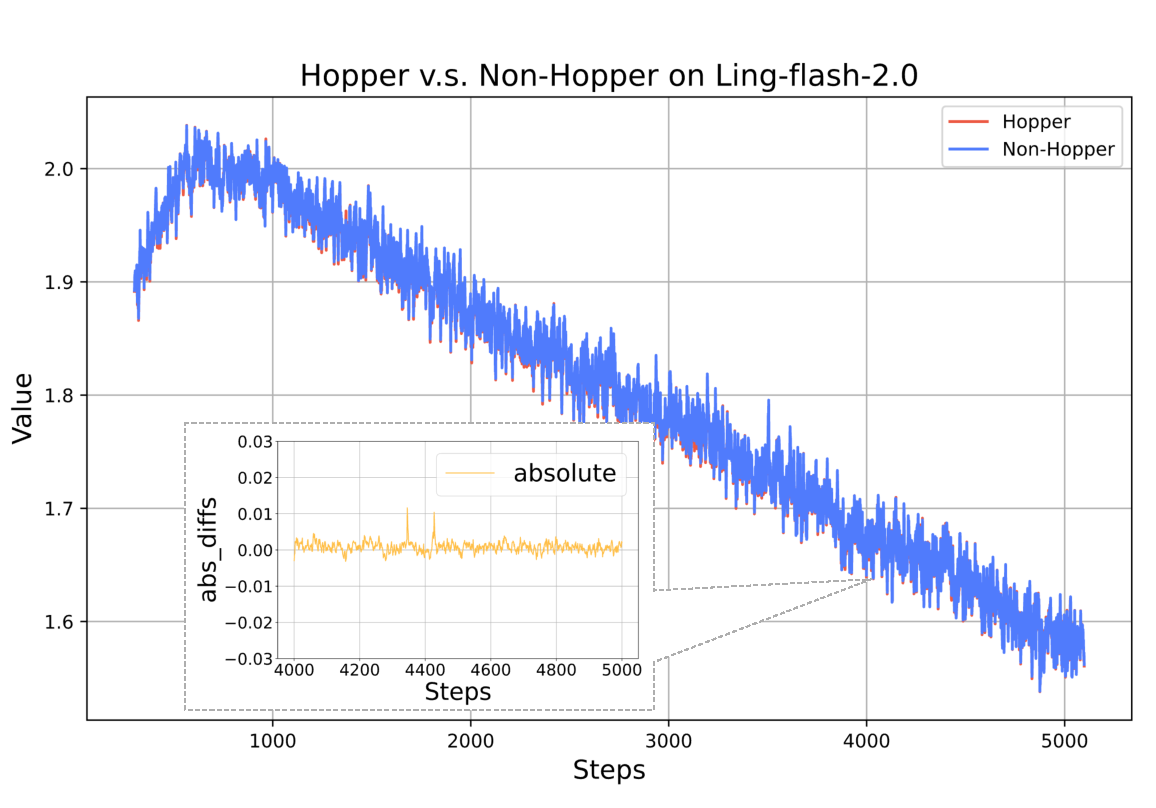
\includegraphics[width=0.57\linewidth]{figs/infra_cross_plat.pdf}
    \caption{The loss comparison of \texttt{Ling-flash-2.0} on Hopper vs. Non-Hopper GPUs.}
    \label{fig:infra_cross_plat}
\end{figure}

Figure~\ref{fig:infra_cross_plat} shows the alignment results based on \texttt{Ling-flash-2.0}. Throughout the training process, the differences in loss values consistently oscillate around zero. This indicates that although variations in operator implementations across different GPU architectures introduce floating-point precision deviations, the mean value of these errors remains within one-thousandth\footnote{The increase in loss curve during the first 1,000 steps was caused by a switch in the training data and the fact that the optimizer state of the model was not loaded.}.
We consider such deviations insufficient to affect the accuracy of model training convergence, thus ensuring the validity of Ling 2.0 series model training on heterogeneous platforms.


\subsection{Evaluation Pipeline}
Model evaluation provides critical insights into model quality and informs continuous algorithmic and engineering optimizations based on feedback. However, at the trillion-parameter scale, traditional evaluation methods face significant challenges in stability, speed, and precision, severely constraining the development and training of  Ling 2.0 models.
To overcome these issues, we redesigned the entire evaluation pipeline based on OpenCompass \citep{2023opencompass} to support large-scale, distributed, and incremental benchmarking. The system now integrates on-the-fly checkpoint evaluation, dynamic resource scheduling, and prompt caching to minimize redundant computation. Compared with the original OpenCompass, the total evaluation time per checkpoint was reduced by more than two-thirds.

\textbf{Multi-Node Inference Optimization.} For large models that cannot fit on a single GPU node, we extended OpenCompass to support distributed evaluation across Ray Clusters. Each evaluation task dynamically allocates multi-node multi-instance resources and interfaces with the SGLang \citep{zheng2024sglang} inference backend for high-throughput serving. This allows us to handle trillion-parameter models with balanced network and GPU utilization.

\textbf{Prompt Caching For Repeated Prefixes.} In benchmark settings that involve repeated prompts (e.g., identical few-shot templates or shared prefixes across options), recomputing log-probabilities (PPL) for each variant is wasteful. We implemented prefix-level caching that reuses the shared prompt embedding across samples, improving evaluation throughput by more than 30\%.

\textbf{Batch Parallelization and Async Execution.} The original OpenCompass implementation handled prompt preprocessing, inference, and postprocessing serially. We parallelized these steps and introduced asynchronous inference scheduling. Small requests are automatically batched into larger groups to increase GPU saturation, improving overall service efficiency and stability.

These optimizations collectively make evaluation a continuous feedback component of training rather than a separate phase. By integrating distributed inference, prompt reuse, and asynchronous batching, we achieved significant improvements in evaluation speed, resource efficiency, and iteration velocity, ensuring that model checkpoints can be validated within hours rather than days.

\subsection{A Bitter Lesson of Computation-Communication Overlapping}

Studies on large MoE models, such as DualPipe and interleaved 1F1B with A2A overlap \citep{deepseekai2024deepseekv3technicalreport,NeMo}, improve training efficiency by overlapping expert computation in one micro-batch with A2A communication in another through modified PP scheduling.
We applied these methods in Ling 2.0 training, and resolving several performance issues, such as streaming multiprocessors (SMs) computation–communication contention and CPU synchronization bottlenecks.
However, the end-to-end acceleration remained limited. We have analyzed the reasons for the lack of significant end-to-end training acceleration despite these fixes. Key factors include:

\begin{itemize}[leftmargin=1.5em]
    \item \textbf{Overlapping Strategy Need a Large EP Configuration:} With fixed resources and global batch size, larger EP size assigns more tokens per expert, boosting expert-layer matrix efficiency while masking added communication overhead. However, EP group time is gated by the slowest rank. The larger EP size reduces experts per rank, exacerbating this bottleneck effect. Additionally, the performance of DeepEP itself is influenced by the balance of token routing.
    \item \textbf{Imbalanced Routing in Shallow MoE Layers:} Routing in the shallow layers of MoE models tends to be more imbalanced, which makes the PP rank containing these layers more prone to OOM errors. This forced us to reconsider the PP partitioning strategy to alleviate the issue, and the new approach incurred an overall performance penalty due to these constraints.
\end{itemize}

In summary, large EP-based optimizations are more sensitive to routing imbalance than smaller configurations.
Although Ling 2.0 training saw limited gains, we view computation–communication overlap as a key avenue for improving large-scale MoE performance and plan to jointly optimize routing and related components to better realize its potential benefits.
